%
% Appendix
%

% !TEX root = ../main.tex

\chapter{Anhang}

  \section{Projektmanagement}
  \begin{landscape}
    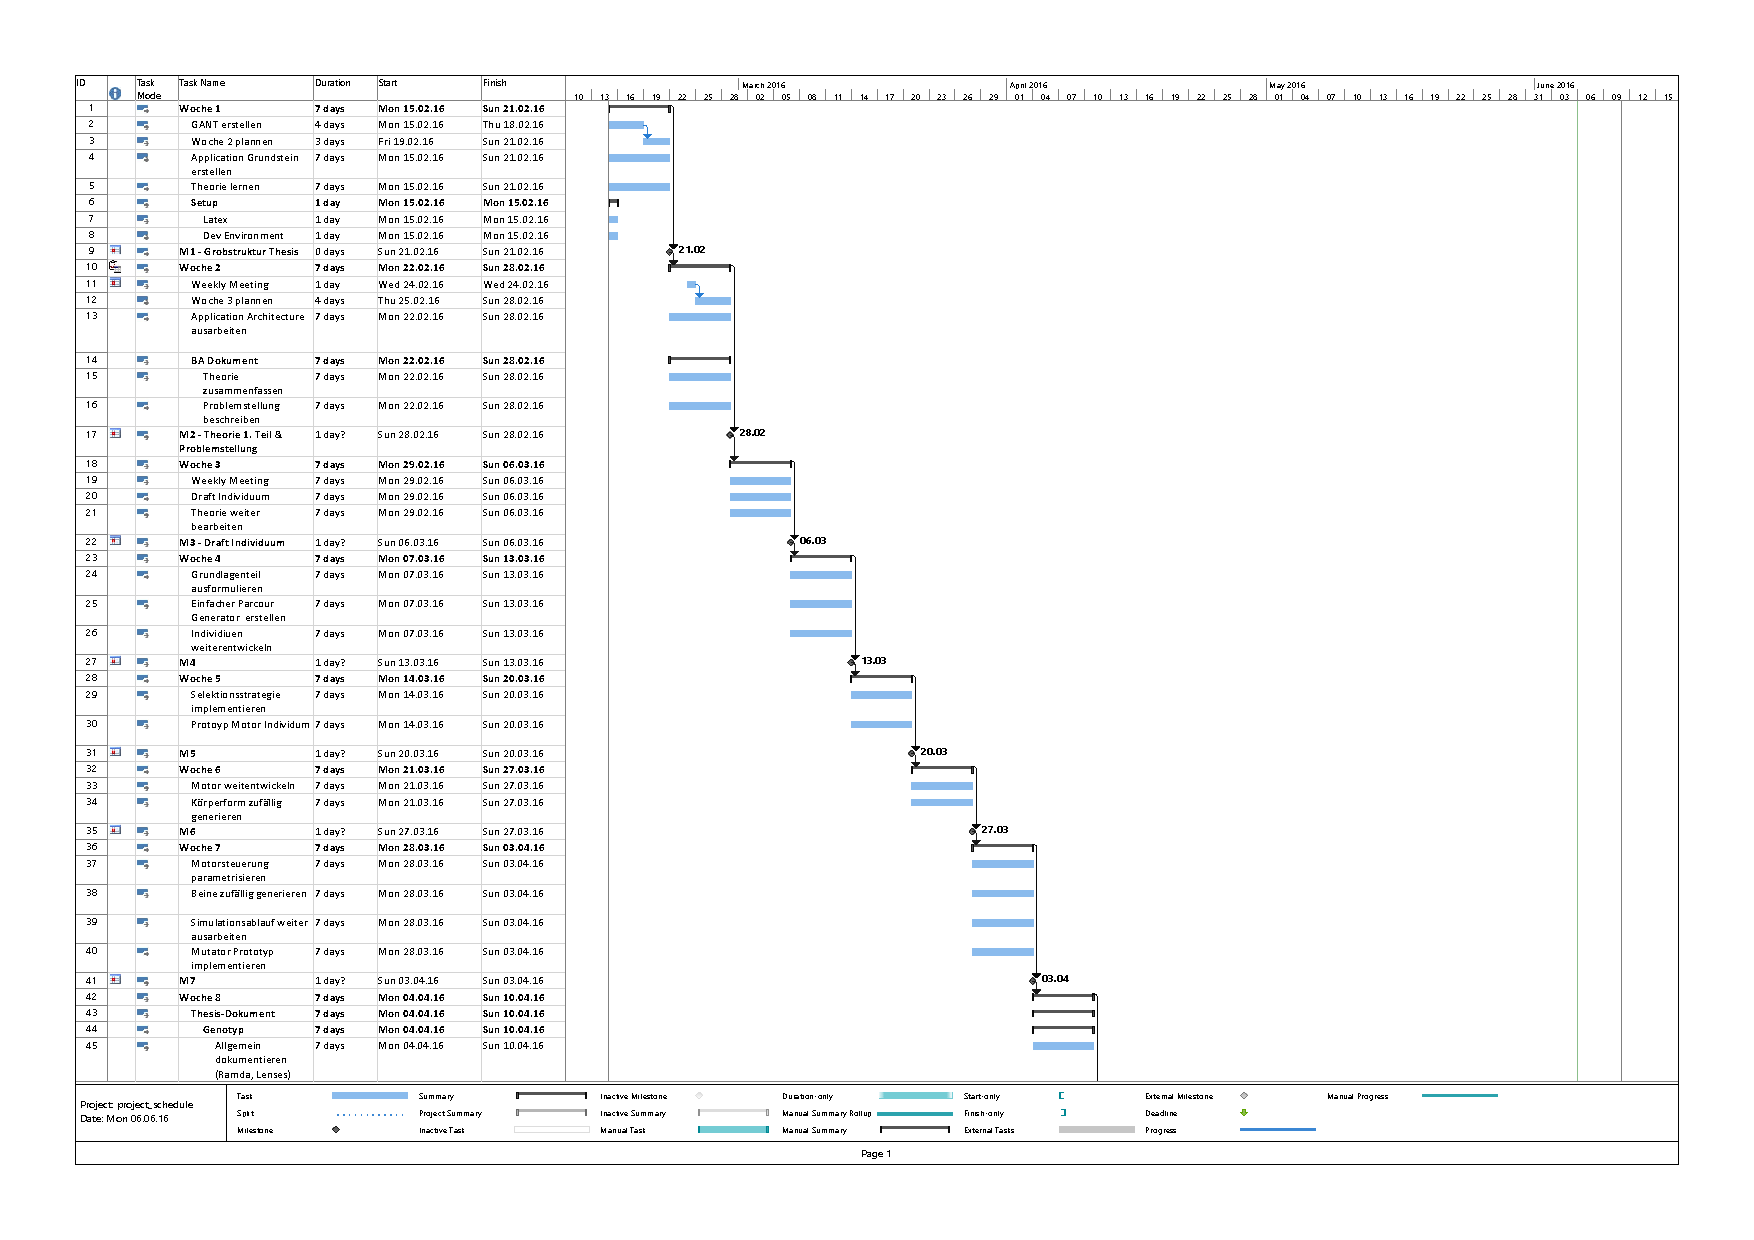
\includepdf[landscape=true]{templates/project_schedule_1.pdf}
  \end{landscape}

    \subsection{Protokolle}

      %
      % includepdf uses intrnally includegraphics.
      % But additionally a new page is inserted.
      % Therefore the page is scaled down to fit on the current page with a heading.
      %
      
\includegraphics[page=1,scale=0.8,trim=20 20 20 20,clip]{templates/protocols}
      
\includepdf[pages=2-last,scale=0.8,trim=20 20 20 20,clip]{templates/protocols}

  \section{Weiteres}
    \todo[inline]{CD mit dem vollständigen Bericht als pdf-File inklusive Film- und Fotomaterial\\
    (Schaltpläne und Ablaufschemata)\\
    (Spezifikationen u. Datenblätter der verwendeten Messgeräte und/oder Komponenten)\\
    (Berechnungen, Messwerte, Simulationsresultate)\\
    (Stoffdaten)\\
    (Fehlerrechnungen mit Messunsicherheiten)\\
    (Grafische Darstellungen, Fotos)\\
    (Datenträger mit weiteren Daten (z. B. Software-Komponenten) inkl. Verzeichnis der auf
    diesem Datenträger abgelegten Dateien)}
